\subsection{Task 2.3 -- Class diagram}

\subsubsection{Mục đích và phạm vi}
Sơ đồ lớp mô tả cấu trúc nghiệp vụ của BrewLite, làm cơ sở tổ chức dữ liệu
cho luồng đặt và thanh toán đồ uống. Mô hình dựa trên SRS, use-case UC-CK
và cách nhận diện lớp của Sommerville (\textit{Software Engineering},
10th Global Edition, mục 5.3 và 7.1.3).
Hình~\ref{fig:class-domain} trình bày các lớp và quan hệ;
Hình~\ref{fig:class-domain-enums} thể hiện các trạng thái và kiểu giá trị.

\subsubsection{Các nhóm lớp}
Mô hình gồm bảy lớp bắt buộc và bốn lớp bổ trợ, được tổ chức thành năm nhóm:

{\small
\begin{tabularx}{\linewidth}{@{}>{\raggedright\arraybackslash}p{0.16\linewidth}>{\raggedright\arraybackslash}p{0.35\linewidth}>{\raggedright\arraybackslash}X@{}}
\toprule
\textbf{Nhóm} & \textbf{Các lớp} & \textbf{Vai trò} \\
\midrule
Người dùng & User & Lưu tài khoản, vai trò và số dư điểm. \\
Đơn hàng & Order, OrderItem & Lưu đơn, tùy chọn món, giá và trạng thái. \\
Món và kho & Product, RecipeItem, Ingredient & Mô tả đồ uống, công thức và nguyên liệu. \\
Thanh toán & Payment, BankTransaction & Quản lý phiên thanh toán và sao kê tiền vào/hoàn tiền. \\
Ưu đãi & Promotion, VoucherUsage, LoyaltyTransaction & Mô tả mã giảm giá, lượt sử dụng và sự kiện điểm. \\
\bottomrule
\end{tabularx}
\par
}

\subsubsection{Quan hệ và ràng buộc nghiệp vụ}
Mỗi Order thuộc một User và chứa ít nhất một OrderItem. Order--OrderItem
là quan hệ thành phần (composition) vì dòng món thuộc vòng đời của đơn. Một đơn có thể có nhiều
Payment qua các lần thử, nhưng tối đa một phiên đang chờ xử lý.
Khóa \texttt{idempotencyKey} của Payment là duy nhất, ngăn tạo phiên trùng khi gửi lại yêu cầu.
BankTransaction luôn gắn với Order và có thể không gắn trực tiếp Payment.
RecipeItem liên kết Product với Ingredient theo định lượng size S;
\texttt{/stock} là số ly suy ra cho size S không topping. Các bội số
\texttt{0..1}, \texttt{0..*}, \texttt{1..*} thể hiện tính tùy chọn và số lượng
đối tượng; dấu \texttt{?} chỉ giá trị có thể để trống.

Mỗi đơn dùng tối đa một mã; mỗi tài khoản/mã có tối đa ba lượt, tính cả lượt
đang giữ và đã dùng.
Nguyên liệu và lượt mã được giữ khi tạo đơn; PAID chốt lượt và cộng điểm,
không trừ kho thêm. PAYMENT\_FAILED chưa hoàn kho; CANCELLED hoàn kho,
trả lượt và thu hồi điểm đã cộng đúng một lần. TRANSFER\_RECEIVED thuộc
Payment; nhân viên mới xác nhận Order PAID. Đơn chưa có tiền về hết hạn sau
15 phút, còn đơn đã có tiền về chờ nhân viên xử lý.

\subsubsection{Ánh xạ với hệ thống hiện tại}
Promotion tương ứng với Voucher trong mã nguồn; \texttt{isPublic} phân biệt
mã có sẵn trong danh sách với mã chỉ nhập trực tiếp. LoyaltyTransaction là lớp
nghiệp vụ suy ra từ Order, chưa có bảng hay API riêng. Với đơn áp dụng chính
sách điểm phiên bản 1, sự kiện EARN được xác định tại pointsAwardedAt với
số điểm bằng \texttt{pointsEarned + pointsReversed}; REVERSAL được xác định
tại pointsReversedAt với số điểm bằng \texttt{-pointsReversed}.
Bội số \texttt{0..2} biểu diễn chưa cộng, đã cộng hoặc đã cộng rồi thu hồi
một lần. Đơn 0 điểm vẫn có mốc xử lý; không tự suy ra sự kiện cho đơn thuộc
chính sách cũ hoặc thiếu mốc. Cách ánh xạ này giữ nhất quán với dữ liệu hiện có.

% The parent report supplies graphicx and, when compiled from the repo root,
% \graphicspath{{docs/diagrams/}}. Image basenames also work in a flat Overleaf upload.
\begin{figure}[p]
  \centering
  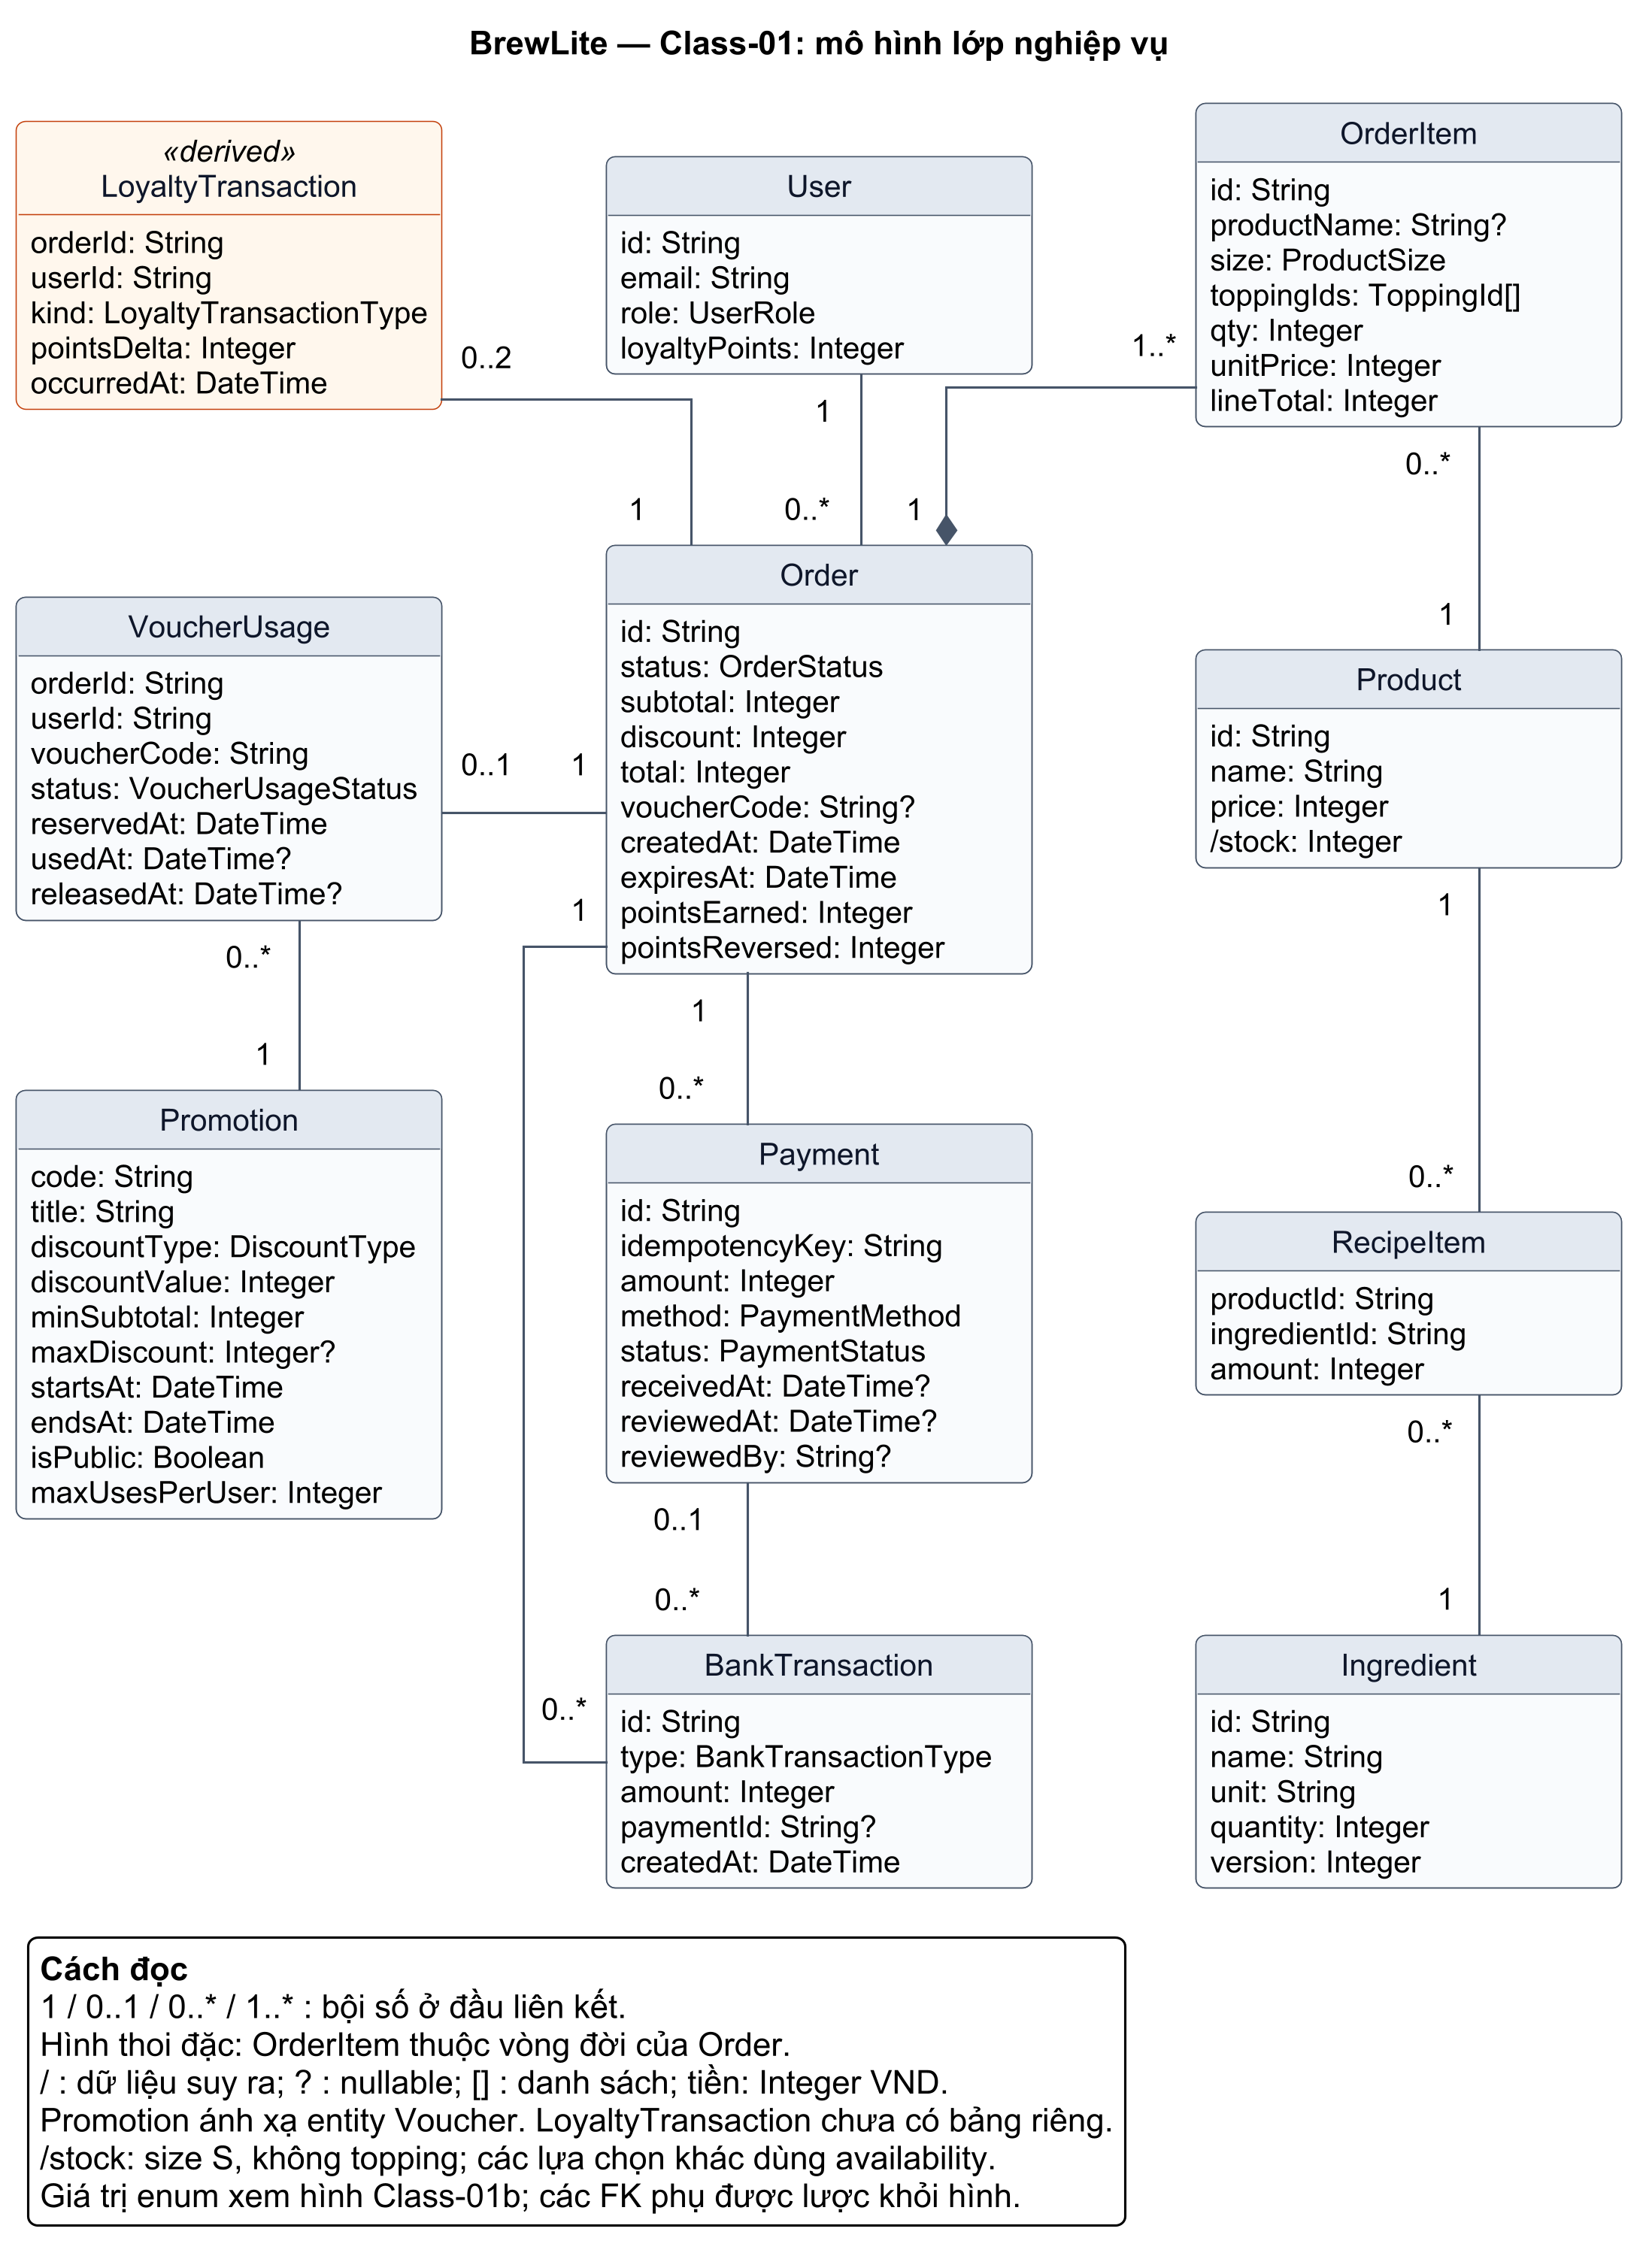
\includegraphics[width=\linewidth,height=0.92\textheight,keepaspectratio]{class-domain.png}
  \caption{Class-01: các lớp nghiệp vụ và bội số liên kết.}
  \label{fig:class-domain}
\end{figure}

\begin{figure}[p]
  \centering
  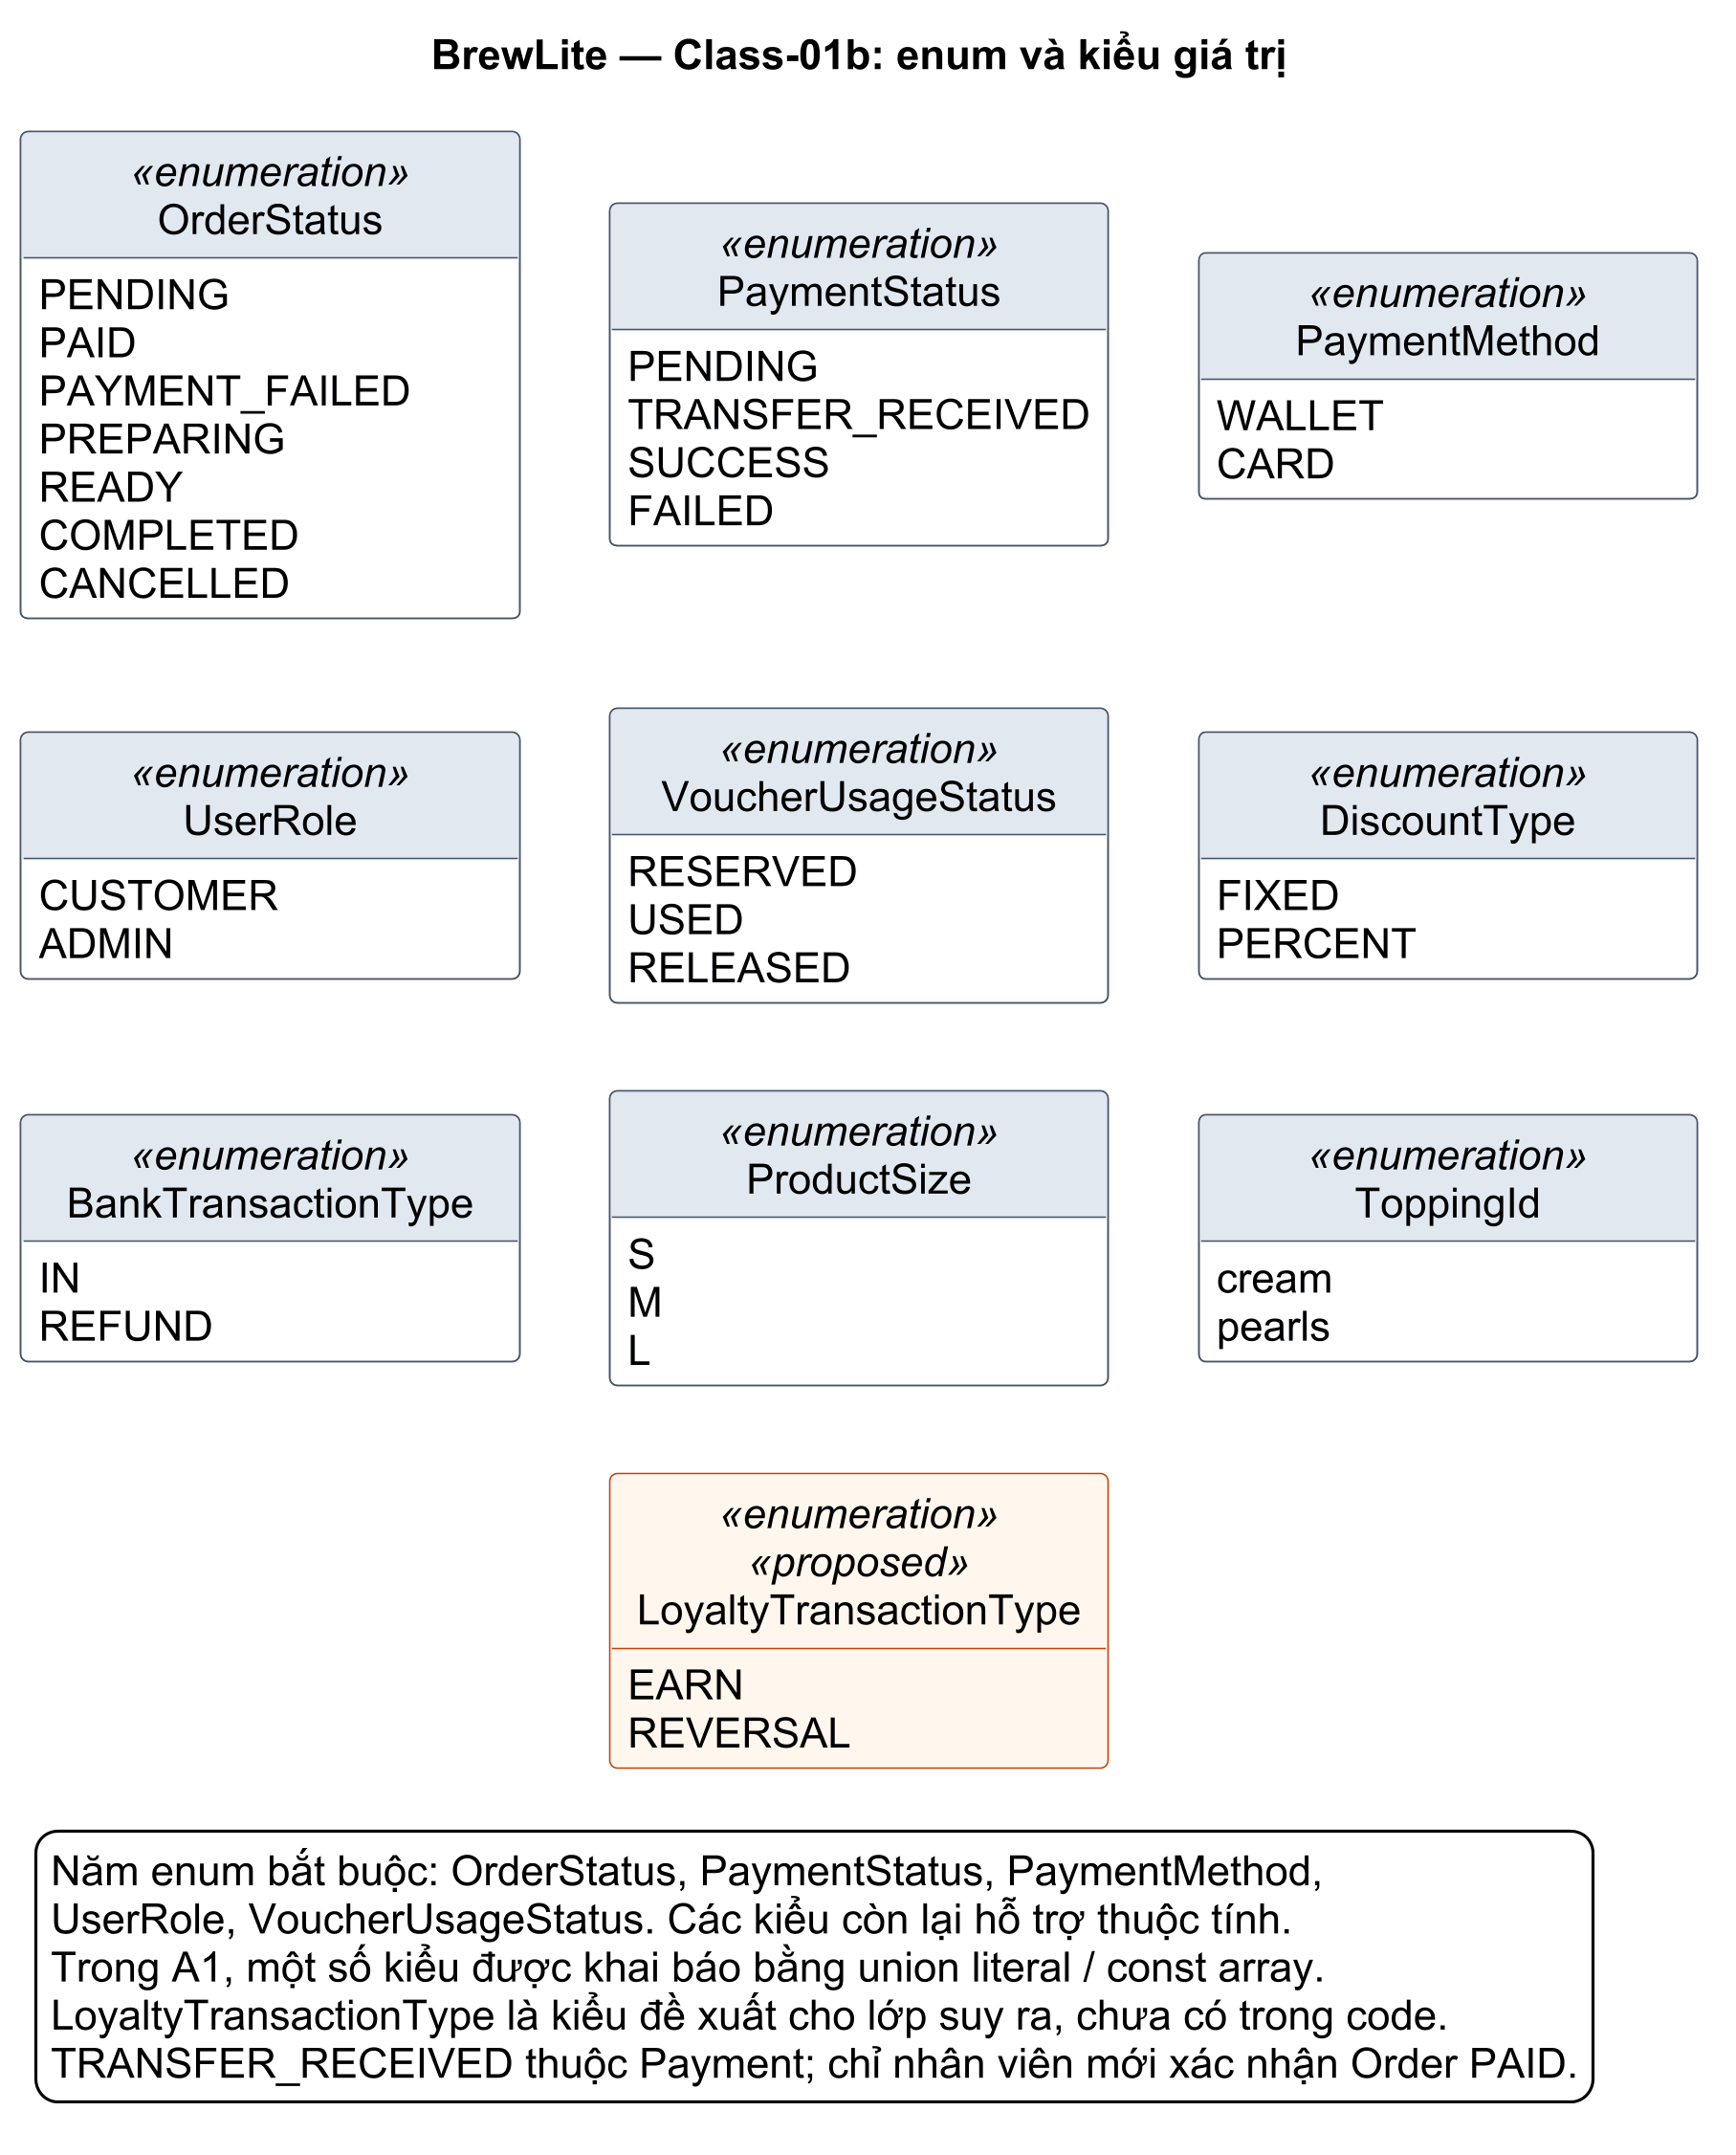
\includegraphics[width=0.95\linewidth,height=0.80\textheight,keepaspectratio]{class-domain-enums.png}
  \caption{Class-01b: enum bắt buộc và các kiểu giá trị bổ trợ của Class-01.}
  \label{fig:class-domain-enums}
\end{figure}
